\documentclass[12pt,fleqn]{article}\usepackage{../../common}
\begin{document}
Radyo Dalgalari

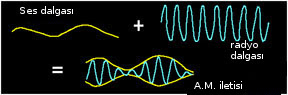
\includegraphics[width=20em]{AM_waves.jpg}

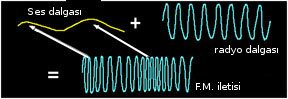
\includegraphics[width=20em]{FM_waves.jpg}

\inputminted[fontsize=\footnotesize]{python}{FMDemodulator.py}

[devam edecek]

Kaynaklar

[1] {\em The Basic Facts About Radio Signals}, \url{https://www.windows2universe.org/spaceweather/wave_modulation.html}

[2] \url{https://www.dropbox.com/s/lpwz2iby0nhh8p7/fm1.dat?dl=1}

[3] \url{https://www.dropbox.com/s/70adji6wyst0qbi/fm2.dat?dl=1}

[4] Scher, {\em How to capture raw IQ data from a RTL-SDR dongle and FM demodulate with MATLAB},\url{http://www.aaronscher.com/wireless_com_SDR/RTL_SDR_AM_spectrum_demod.html}

[5] {\em EE123: Digital Signal Processing}, \url{http://inst.eecs.berkeley.edu/~ee123/sp14/}

[6] Fund, {\em Capture and decode FM radio}, \url{https://witestlab.poly.edu/blog/capture-and-decode-fm-radio/}

[7] Fund, {\em Lab 1: Working with IQ data in Python}, \url{http://witestlab.poly.edu/~ffund/el9043/labs/lab1.html}

\end{document}




















